\documentclass[12pt]{article}
\usepackage[top=1in,bottom=1in,left=0.75in,right=0.75in,centering]{geometry}
\usepackage{fancyhdr}
\usepackage{epsfig}
\usepackage[pdfborder={0 0 0}]{hyperref}
\usepackage{palatino}
\usepackage{wrapfig}
\usepackage{lastpage}
\usepackage{color}
\usepackage{ifthen}
\usepackage[table]{xcolor}
\usepackage{graphicx,type1cm,eso-pic,color}
\usepackage{hyperref}
\usepackage{amsmath}
\usepackage{wasysym}
\usepackage{amsfonts}

\def\course{CS 3120: Discrete Math and Theory II}
\def\homework{Set Cardinality}
\def\semester{Spring 2024}

\newboolean{solution}
\setboolean{solution}{false}

% add watermark if it's a solution exam
% see http://jeanmartina.blogspot.com/2008/07/latex-goodie-how-to-watermark-things-in.html
\makeatletter
\AddToShipoutPicture{%
\setlength{\@tempdimb}{.5\paperwidth}%
\setlength{\@tempdimc}{.5\paperheight}%
\setlength{\unitlength}{1pt}%
\put(\strip@pt\@tempdimb,\strip@pt\@tempdimc){%
\ifthenelse{\boolean{solution}}{
\makebox(0,0){\rotatebox{45}{\textcolor[gray]{0.95}%
{\fontsize{5cm}{3cm}\selectfont{\textsf{Solution}}}}}%
}{}
}}
\makeatother

\pagestyle{fancy}

\fancyhf{}
\lhead{\course}
\chead{Page \thepage\ of \pageref{LastPage}}
\rhead{\semester}
%\cfoot{\Large (the bubble footer is automatically inserted into this space)}

\setlength{\headheight}{14.5pt}

\newenvironment{itemlist}{
\begin{itemize}
\setlength{\itemsep}{0pt}
\setlength{\parskip}{0pt}}
{\end{itemize}}

\newenvironment{numlist}{
\begin{enumerate}
\setlength{\itemsep}{0pt}
\setlength{\parskip}{0pt}}
{\end{enumerate}}

\newcounter{pagenum}
\setcounter{pagenum}{1}
\newcommand{\pageheader}[1]{
\clearpage\vspace*{-0.4in}\noindent{\large\bf{Page \arabic{pagenum}: {#1}}}
\addtocounter{pagenum}{1}
\cfoot{}
}

\newcounter{quesnum}
\setcounter{quesnum}{1}
\newcommand{\question}[2][??]{
\begin{list}{\labelitemi}{\leftmargin=2em}
\item [\arabic{quesnum}.] {} {#2}
\end{list}
\addtocounter{quesnum}{1}
}


\definecolor{red}{rgb}{1.0,0.0,0.0}
\newcommand{\answer}[2][??]{
\ifthenelse{\boolean{solution}}{
\color{red} #2 \color{black}}
{\vspace*{#1}}
}

\definecolor{blue}{rgb}{0.0,0.0,1.0}

\begin{document}

\section*{\homework}


\question[3]{
For each of the following claims, state whether it is true or false and then prove your assertion.
}

\begin{itemize}
	\item All finite sets have an \emph{injection} to $\mathbb{N}$
	\item All finite sets have a \emph{surjection} to $\mathbb{N}$
	\item If $A$ is a countably infinite set (i.e., $|A|=|\mathbb{N}|$) and $B$ is a also a countably infinite set (i.e., $|B| = |\mathbb{N}|$), then $A \cup B$ is also countable.
	\item If $A$ is countably infinite and $B$ is uncountably infinite, then $A \cup B$ is countable.
	\item If $A$ is countably infinite and $B$ is uncountably infinite, then $A \cap B$ is countable.
\end{itemize}

\vspace{12pt}



\question[3]{
Consider a square grid with length and width $n$. The bottom left corner is considered position $(0,0)$ and the upper right corner is position $(n,n)$ \emph{(*Note that the first item in the tuple is the square along the horizontal axis and the second element is the index along the vertical axis)}. You can see an example grid below.\\
\\
Our goal is to count the number of unique ways a robot starting at cell $(0,0)$ can reach cell $(n,n)$ by only moving up or to the right on each individual move. You need to do two things: 1) Prove that the number of unique moves is equal to the number of binary bitstrings of length $2n$ that contain exactly $n$ 1's by describing a bijection between these two sets. Then, 2) Declare how many unique moves this is as a function of $n$.
}

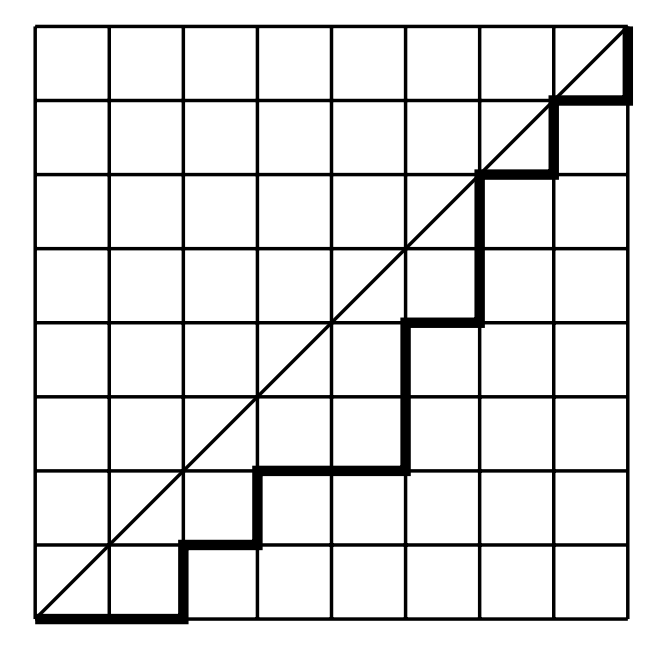
\includegraphics[scale=0.4]{img/lattice}

\vspace{12pt}

\question[3]{
Use a proof by diagonalization to show that the following set is uncountable:\\
\\
$F=\{ f:\mathbb{N} \rightarrow \mathbb{N} | (a>b) \rightarrow (f(a) > f(b)) \}$
\\
\\
In other words, this is the set of all strictly increasing functions that map natural numbers to natural numbers. A function is strictly increasing if larger inputs are guaranteed to produce larger outputs.\\
\\
For example, $f(x)=x^2$ is strictly increasing since if $a>b$, then $a^2>b^2$. However, $f(x)=(x-5)^2$ is not strictly increasing since $1<2$ but $f(1) > f(2)$.
}

\vspace{12pt}



\end{document}
